\documentclass[a4paper,11pt]{article}
\usepackage[utf8]{inputenc}
\usepackage[spanish]{babel}
\usepackage[affil-it]{authblk}
\usepackage{enumerate}
\usepackage{graphicx}
\usepackage{hyperref}
\usepackage{amsmath}
\usepackage{amssymb}
\usepackage{cancel}
\usepackage[usenames, dvipsnames]{color}
\usepackage{tikz}
\usepackage[labelfont=bf]{caption}
\usepackage{subcaption} %Multiple images
\usepackage{multicol} % Multiple columns
\usepackage{float}
\usepackage{cleveref}
\usepackage{relsize} % bigger math symbols
\usepackage[margin=1.1in]{geometry}
\usepackage[titletoc,toc,title]{appendix}
\usepackage{enumitem}
\usepackage{etoolbox}
\usepackage{mdframed} %frame theorems
\usetikzlibrary{calc}
\numberwithin{equation}{section}

% Footnotes with symbols

\makeatletter
\def\@fnsymbol#1{\ensuremath{\ifcase#1\or \dagger\or \ddagger\or
   \mathsection\or \mathparagraph\or \|\or **\or \dagger\dagger
   \or \ddagger\ddagger \else\@ctrerr\fi}}
\makeatother

\renewcommand{\thefootnote}{\fnsymbol{footnote}}

% Cool letters 
%Filename:      Typocaps.fd
%Created by:    MLO
%Creation date: 2003/04/02

% This file should be put in a TeX input directory

\ProvidesFile{Typocaps.fd}
   [2003/04/02 Font definition file for U/Typocaps]

\DeclareFontFamily{U}{Typocaps}{}

\DeclareFontShape{U}{Typocaps}{xl}{n}{
   <-> Typocaps
}{}

\endinput


% Footer
\usepackage{fancyhdr}
\pagestyle{fancy}
\fancyhf{}
\cfoot{\fontsize{15pt}{15pt}\usefont{U}{Typocaps}{xl}{n} 
gigantium humeris insidentes}

% Big Pictures
\usepackage[export]{adjustbox}

% Enviroment for theorems
\newmdtheoremenv[frametitle=Teorema]{theo}{Theorem}

% Circled words
\newcommand{\circled}[2][]{%
  \tikz[baseline=(char.base)]{%
    \node[shape = circle, draw, inner sep = 1pt]
    (char) {\phantom{\ifblank{#1}{#2}{#1}}};%
    \node at (char.center) {\makebox[0pt][c]{#2}};}}
\robustify{\circled}

%Appendices in spanish
\renewcommand{\appendixname}{Ap\'endices}
\renewcommand{\appendixtocname}{Ap\'endices}
\renewcommand{\appendixpagename}{Ap\'endices}

%Zero delimiter
\newcommand{\zerodel}{.\kern-\nulldelimiterspace}

%Columns separation
\setlength{\columnsep}{1cm}

%Indentation
\setlength{\parindent}{0ex}

%Multiple References

\crefrangelabelformat{equation}{(#3#1#4--#5\crefstripprefix{#1}{#2}#6)}

\usepackage{xparse}

%Boxes

\newcommand*{\boxcolor}{blue}
\makeatletter
\renewcommand{\boxed}[1]{\textcolor{\boxcolor}{%
\tikz[baseline={([yshift=-1ex]current bounding box.center)}] \node [rectangle, minimum width=1ex,rounded corners,draw] {\normalcolor\m@th$\displaystyle#1$};}}
 \makeatother

%Constantes
\newcommand{\euler}{\mathrm{e}}
\newcommand{\im}{i}

%Lemas, teoremas, definiciones y pruebas
\newcommand{\definicion}{\textbf{Definición: }}
\newcommand{\lema}{\textbf{Lema: }}
\newcommand{\teorema}{\textbf{Teorema: }}
\newcommand{\prueba}{\textbf{Prueba: }}
\newcommand{\proposicion}{\textbf{Proposición: }}
\newcommand{\corolario}{\textbf{Corolario: }}

% Definición de las secciones y su numeración

\makeatletter
\def\@seccntformat#1{%
  \expandafter\ifx\csname c@#1\endcsname\c@section\else
  \csname the#1\endcsname\quad
  \fi}
\makeatother

\begin{document}

\begin{titlepage}
\thispagestyle{fancy}

\newcommand{\HRule}{\rule{\linewidth}{0.5mm}} % Defines a new command for the horizontal lines, change thickness here

\center % Center everything on the page
 
%----------------------------------------------------------------------------------------
%	HEADING SECTIONS
%----------------------------------------------------------------------------------------

\textsc{\LARGE Universidad Nacional Autónoma de México}\\[0.3cm] % Name of your university/college

%----------------------------------------------------------------------------------------
%	LOGO SECTION
%----------------------------------------------------------------------------------------


\includegraphics[scale=0.17]{unam}

%----------------------------------------------------------------------------------------
%	SUBHEADING SECTIONS
%----------------------------------------------------------------------------------------

\textsc{\Large Electrodinámica Clásica}\\[0.3cm] % Major heading such as course name
\textsc{\large Semestre 2016-II}\\[0.3cm] % Minor heading such as course title
\textsc{\large 7 de abril de 2016}\\ % Minor heading such as course title

%----------------------------------------------------------------------------------------
%	TITLE SECTION
%----------------------------------------------------------------------------------------

\HRule \\[0.1cm]
{ \huge \bfseries Tarea \# 6. \\ Ondas electromagnéticas planas \\
y propagación de ondas.}\\ % Title of your document
\HRule \\[0.1cm]
 
%----------------------------------------------------------------------------------------
%	AUTHOR SECTION
%----------------------------------------------------------------------------------------
\setcounter{footnote}{0}
\center
\large
\emph{Autor:} \\ % Your name
\Large Favio \textsc{Vázquez}\footnote[1]{\href{mailto:favio.vazquez@correo.nucleares.unam.mx}{favio.vazquez@correo.nucleares.unam.mx}}
\\[0.7cm]
%----------------------------------------------------------------------------------------
%	COOL IMAGE SECTION
%----------------------------------------------------------------------------------------

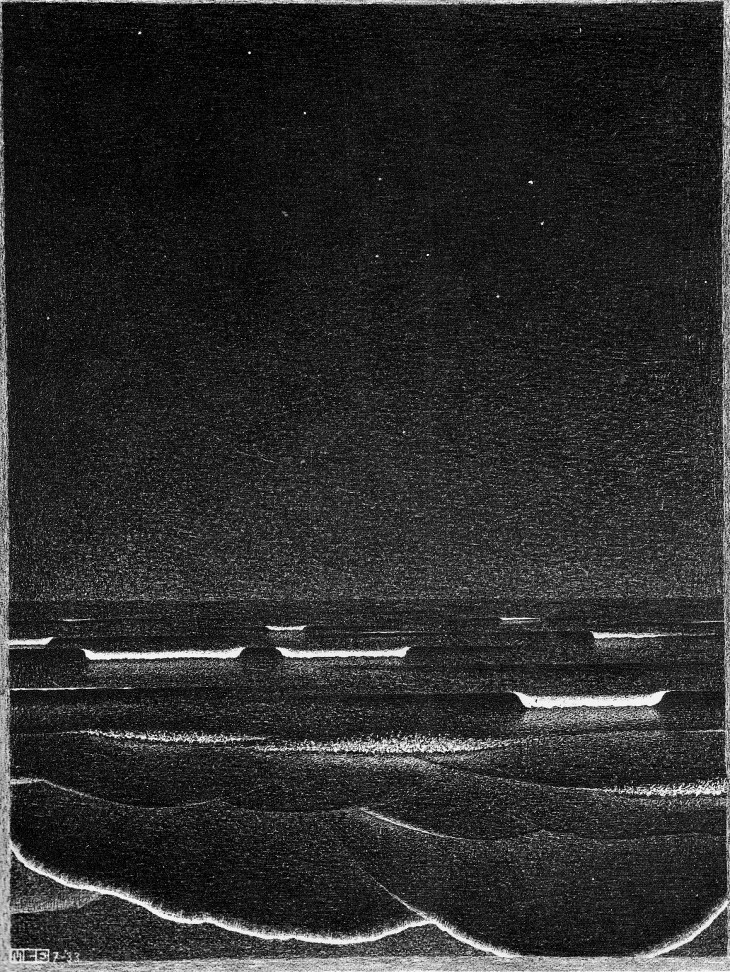
\includegraphics[scale=1.2]{escherOndas}

%----------------------------------------------------------------------------------------

\vfill % Fill the rest of the page with whitespace

\end{titlepage}

% ---------------------------------------------------------------------------------------
%         HEADER
%----------------------------------------------------------------------------------------

\fancyhead[L]{Favio Vázquez}
\fancyhead[R]{\thepage}

%----------------------------------------------------------------------------------------
\setcounter{footnote}{0}
\renewcommand*{\thefootnote}{\arabic{footnote}}
%----------------------------------------------------------------------------------------

%----------------------------------------------------------------------------------------
%%			BEGIN DOCUMENT
%----------------------------------------------------------------------------------------

\section{Problema 1. Problema 7.2 de Classical Electromagnetic Radiation
de Jackson \cite{jackson}.}

Una onda plana incidente en una interfaz de capas como se muestra en la figura. Los 
índices de refracción de los tres medios no impermeables son $n_1$, $n_2$ y $n_3$. 
El grosor de la capa intermedia es $d$. Cada uno de los otros medios es semi-infinito.

\begin{enumerate}[label=\textbf{(\alph*)}]
 \item Calcule los coeficientes de transmisión y reflexión (las tasas de del flujo de 
 Poynting transmitida y reflejada al flujo incidente), y esboce su comportamiento como 
 función de la frecuencia para $n_1 = 1$, $n_2 = 2$, $n_3 = 3$; $n_1 = 3$, $n_2 = 2$, 
 $n_3 = 1$ y $n_1 = 2$, $n_2 = 4$, $n_3 = 1$.

\begin{figure}[H]
 \center 
 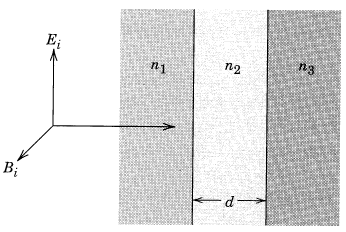
\includegraphics[scale=0.7]{problema1fig1}
\end{figure}

\item El medio $n_1$ es parte de un sistema óptico (e.g., una lente); el medio 
$n_3$ es aire $(n_3 = 1)$. Se desea colocar un revestimiento óptico (medio $n_2$) 
sobre la superficie para que no haya reflexión para ondas de frecuencia $\omega_0$. 
¿Qué grosor $d$ e índice de refracción $n_2$ son necesarios?

\end{enumerate}

\vspace{.3cm}

\underline{Solución:} \vspace{.3cm}

\newpage

\section{Problema 2. Problema 7.3 de Classical Electromagnetic Radiation
de Jackson \cite{jackson}.}

Dos losas planas semi-infinitas con el mismo dieléctrico sin pérdidas, uniformidad,
isotropía, no-permeabilidad con índice de refracción $n$ son paralelas, y están 
separadas por una brecha de aire ($n = 1$) de ancho $d$. Una onda electromagnética 
de frecuencua $\omega$ incide en la brecha desde una de las losas con un ángulo 
de incidencia $i$. Para una polarización lineal tanto paralela como perpendicular 
al plano de incidencia,

\begin{enumerate}[label=\textbf{(\alph*)}]
 \item calcule la tasa de potencia transmitida a la segunda losa con respecto 
 al poder incidente y la tasa de poder reflejado con respecto al incidente;
 \item para un $i$ mayor que el ángulo crítico para reflexión interna total, 
 esboce la tasa de potencia transmitida con respecto a la potencia incidente 
 como una función de $d$ medido en unidades de longitud de onda en la brecha.
\end{enumerate}

\vspace{.3cm}

\underline{Solución:} \vspace{.3cm}

\newpage

\section{Problema 3. Problema 7.5 de Classical Electromagnetic Radiation
de Jackson \cite{jackson}.}

Una onda electromagnética polarizada $\mathbf{E} = \mathbf{E}_i \euler^{i\mathbf{k}} 
\cdot \mathbf{x} - i\omega t$ incide normalmente sobre una lámina plana uniforme 
de una excelente conducción ($\omega \gg \omega \epsilon_0$) con un grosor de $D$. 
Asumiendo que en el espacio y en la lámina conductora $\mu/\mu_0 = \epsilon/\epsilon_0 
= 1$, discuta la reflexión y transmisión de la onda incidente. 

\begin{enumerate}[label=\textbf{(\alph*)}]
 \item Muestre que las amplitudes de las onda reflejada y transmitida, correctas 
 a primer orden en $(\epsilon_0 \omega /\sigma)^1/2)$, son 
 
 $$
 \frac{E_r}{E_i} = \frac{-(1 - \euler^{-2\lambda})}{(1 - \euler^{-2\lambda}) 
 + \gamma(1 + \euler^{-2\lambda})}
 $$
 
  $$
 \frac{E_t}{E_i} = \frac{2\gamma \euler^{-\lambda}}{(1 - \euler^{-2\lambda}) 
 + \gamma(1 + \euler^{-2\lambda})}
 $$
 
 donde 
 
 $$
 \gamma = \sqrt{\frac{2\epsilon_0 \omega}{\sigma}}(1 - i) = \frac{\omega \delta}{c}
 (1 - i)
 $$
 
 $$
 \lambda = (1-i)D/\delta
 $$
 
  y $\delta = \sqrt{2/\omega \mu \sigma}$ es la profundidad de penetración.
 
 \item Verifique que para un grosor igual a cero y un grosor infinito se obtienen 
 los resultados limitantes apropiados.
 \item Muestre que, excepto para láminas de muy poco grosor, el coeficiente de 
 transmisión es 
 
 $$
 T = \frac{8(\text{Re} \gamma)^2 \euler^{-2D/\gamma}}{1 - 2\euler^{-2D/\gamma} 
 \cos{2D/\delta) + \euler^{-4/\gamma}}}
 $$
\end{enumerate}

Esboce log $T$ como una función de $(D/\delta)$, asumiendo que Re $\gamma = 10^{-2}$. 
Defina ``grosor muy pequeño''.

\vspace{.3cm}

\underline{Solución:} \vspace{.3cm}

\newpage

\section{Problema 4. Problema 7.14 de Classical Electromagnetic Radiation
de Jackson \cite{jackson}. (Es el 7.9 de la 2da ed.)}

Un modelo simple para la propagación de ondas de radio en la atmósfera de la 
Tierra o ionosfera consiste en una tierra plana en $z = 0$ y un medio no 
uniforme con $\epsilon = \epsilon(z)$ para $z > 0$. Considere la ecuaciones 
de Maxwell bajo la suposición de que los campos son independientes de $y$ y 
pueden escribirse como funciones de $z$ por $\euler^{i(kx - \omega t)}$. 

\begin{enumerate}[label=\textbf{(\alph*)}]
 \item Muestre que la ecuación de onda que gobierna la propagación para $z > 0$ 
 es 
 
 $$
 \frac{d^2 F}{dz^2} + q^2(z) F = 0,
 $$
 
 donde 
 
 $$
 q^2(z) = \omega^2 \mu_0 \epsilon(z) - k^2
 $$
 
 y $F = E_y$ para la polarización \emph{horizontal}, y 
 
 $$
 q^2(z) = \omega^2 \mu_0 \epsilon(z) + \frac{1}{2\epsilon}\frac{d^2 \epsilon}{dz^2} 
 - \frac{3}{4\epsilon^2}\left(\frac{d \epsilon}{d z} \right)^2 - k^2
 $$
 
 con $F = \sqrt{\epsilon/\epsilon_0}E_z$ para la polarización \emph{vertical}.
 
 \item Use la aproximación WKB para tratar la propagación de ondas dirigidas 
 verticalmente hacia la ionosfera ($k = 0$), asumiendo que la constante dieléctrica 
 está dad por (7.59) con una frecuencia de plasma $\omega_p(z)$ gobernada por una 
 densidad electrónica como se muestra en la figura 7.11. Verifique que los argumentos 
 cualitativos de la sección 7.6 se mantienen, con discrepancias en detalle solo 
 para $\omega ~ \omega_{p,\text{max}}$.
 
 \item Usando los resultados WKB de la parte (b) y los conceptos de propagación 
 de un pulso de la sección 7.8, define una altura efectiva de la ionosfera $h'(\omega)$ 
 calculando el tiempo $T$ para un pulso de frecuencia dominante $\omega$ que viaja 
 hacia arriba y se refleja ($h' \equiv cT/2)$. [La aproximación WKB es discutida 
 en la mayoría de los libros de mecánica cuántica].
\end{enumerate}

\vspace{.3cm}

\underline{Solución:} \vspace{.3cm}

\newpage

\begin{thebibliography}{10}
\bibitem{jackson}
J. Jackson, \emph{Classical Electrodynamics}, 3ra edición. John Wiley and Sons, Inc. 
1999.
\bibitem{griffiths}
D. Griffiths, \emph{Indtroduction to Electrodynamics}, 4ta edición. Pearson, 2013.
\end{thebibliography}

\end{document}